
\def\mytitle{CIRCLE ASSIGNMENT}
\def\myauthor{Jyothsna Paluchuri}
\def\contact{jyothsnapaluchuri07@gmail.com}
\def\mymodule{Future Wireless Communication (FWC)}
\documentclass[10pt, a4paper]{article}
\usepackage[a4paper,outer=1.5cm,inner=1.5cm,top=1.75cm,bottom=1.5cm]{geometry}
\twocolumn
\usepackage{graphicx}
\graphicspath{{./images/}}
\usepackage[colorlinks,linkcolor={black},citecolor={blue!80!black},urlcolor={blue!80!black}]{hyperref}
\usepackage[parfill]{parskip}
\usepackage{lmodern}
\usepackage{tikz}
	\usepackage{physics}
%\documentclass[tikz, border=2mm]{standalone}
%\usepackage{karnaugh-map}
%\documentclass{article}
\usepackage{tabularx}
%\usepackage{circuitikz}
\usepackage{enumitem}
\usetikzlibrary{calc}
\usepackage{amsmath}
\usepackage{amssymb}
\renewcommand*\familydefault{\sfdefault}
\usepackage{watermark}
\usepackage{lipsum}
\usepackage{xcolor}
\usepackage{listings}
\usepackage{float}
\usepackage{titlesec}
\providecommand{\mtx}[1]{\mathbf{#1}}
\titlespacing{\subsection}{1pt}{\parskip}{3pt}
\titlespacing{\subsubsection}{0pt}{\parskip}{-\parskip}
\titlespacing{\paragraph}{0pt}{\parskip}{\parskip}
\newcommand{\figuremacro}[5]{
    \begin{figure}[#1]
        \centering
        \includegraphics[width=#5\columnwidth]{#2}
        \caption[#3]{\textbf{#3}#4}
        \label{fig:#2}
    \end{figure}
}

\newcommand{\myvec}[1]{\ensuremath{\begin{pmatrix}#1\end{pmatrix}}}
\let\vec\mathbf
\lstset{
frame=single, 
breaklines=true,
columns=fullflexible
}
\thiswatermark{\centering \put(181,-119.0){
\includegraphics[scale=0.13]{iith_logo3}} }
\title{\mytitle}
\author{\myauthor\hspace{1em}\\\contact\\FWC22059\hspace{6.5em}IITH\hspace{0.5em}\mymodule\hspace{6em}Assignment}
\begin{document}
	\maketitle
	\tableofcontents
   \section{Problem}
  If the chord y=mx+1 of the circle $x^2+y^2=1$ subtends an angle of measures 45$^{\circ}$ at the major segment of the circle then find the value of m
\section{Construction}
  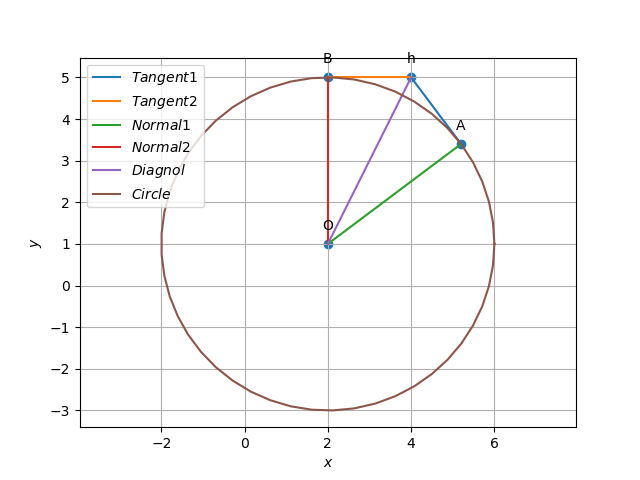
\includegraphics[scale=0.4]{circle.png}
  	\begin{center}
  Figure of construction
  	\end{center}
  \section{Solution}
\textbf{Step1:}
The equation of a line given as
\begin{align}
\implies\vec{n}^T\vec{X} &= c
\end{align}
\begin{align}
\implies\begin{pmatrix}-m & 1 \\ \end{pmatrix}\vec{X}=1
\end{align}

\textbf{Step2:}
The foot of perpendicular from O to the line is given by
\begin{align}
\implies\begin{pmatrix}\vec{m} & \vec{n} \\ \end{pmatrix}^T\vec{X} &= \begin{pmatrix}\vec{m}^T\vec{O} \\ c \\ \end{pmatrix}
\end{align}
\begin{align}
\implies\begin{pmatrix}1 & -m \\m & 1 \\ \end{pmatrix}^T\vec{X} &= \begin{pmatrix}0 \\ 1 \\ \end{pmatrix}
\end{align}

from solving eq (4),we get
\begin{align}
\implies\vec{X} &= \begin{pmatrix}0 \\ 1/m \\ \end{pmatrix}
\end{align}

\textbf{Step3:}
from eq (2) and (5),we get
\begin{align}
\implies\begin{pmatrix}-m & 1 \\ \end{pmatrix}\begin{pmatrix}0 \\ 1/m \\ \end{pmatrix} &= 1
\end{align}
The value of m is
\begin{align}
	\boxed{m=1}
\end{align}	

Get the python code of the figures from
\begin{table}[h]
\large
\centering
\framebox{
\url{https://github.com/jyothsna777/jyothsna-fwc.git}}
\bibliographystyle{ieeetr}
\end{table}

\textbf{termux commands :}
\begin{lstlisting}
bash rncom.sh............using shell command
\end{lstlisting}

\end{document}
